\chapter{Rotational Mechanics}
	\section{Angular Velocity and Acceleration}
	An object that is spinning can be described using angular velocity and angular acceleration.  Angular velocity is a way of expressing how much an object rotates in a given time.  It could be measured in Rotations per Minute (rpms), Degrees per hour, or any other measurement of an angle divided by any measurement of time.  However, it is advantageous to use Radians per Second.
	
	  Just like velocity measures how fast an object is moving in a line, angular velocity measures how fast an object is rotating.    Average angular velocity is given by the following equation:
	  	\begin{mdframed}[backgroundcolor=orange!20!white]
	  \begin{equation}
		\vec{\omega}_{avg} = \frac{\Delta \vec{\theta}}{\Delta t}
	  \end{equation}
	\end{mdframed}
	and instantaneous angular velocity is given by: 
	  	\begin{mdframed}[backgroundcolor=orange!20!white]
	\begin{equation}
	\vec{\omega} = \frac{d \vec{\theta}}{d t}
	\end{equation}
\end{mdframed}


	\section{Angular Kinematics}
	\newpage
	\section{Moment of Inertia}
	\index{Moment of Inertia} \index{Inertia, Moment of} \index{rotational inertia}
	The \textbf{Moment of Inertia} (sometimes called \textbf{rotational inertia}), symbolized $I$, of an object can be thought of as the rotational equivalent of mass.  An object of lesser mass will accelerate more than an object of greater mass when the same amount of force is applied.  Likewise, an object with a smaller moment of inertia will tend to have a greater angular acceleration than an object with a greater moment of inertia when the same forces are applied to the objects.  
	
	The moment of inertia of an object depends both on the mass of the object and the way in which the mass is distributed.  Some common moments of inertia can be found in the attached table.  
	
	\newpage 
	
	
	
	\section{Torque}
	\index{Torque}
	\textbf{Torque} is the rotational equivalent to force.  That is, it is a force that is applied to an object somewhere other than the center of mass, causing the object to rotate.  
	
	
		\begin{mdframed}[backgroundcolor=orange!20!white]
		\begin{equation}
			\vec{\tau} = \vec{r} \times \vec{F}
			\label{equation:torque}
		\end{equation}
	\end{mdframed}
	
	
	You may note that the two vectors are multiplied as a cross product.  The magnitude of the torque is given by:
	
		\begin{mdframed}[backgroundcolor=orange!20!white]
		\begin{equation}
			|\vec{\tau}| = r \cdot F \cdot sin (\theta)
			\label{equation:torquemagnitude}
		\end{equation}
	\end{mdframed}
	
	and the direction is given by the 1st Right Hand Rule (see \cref{RHR1}).
	
	\begin{mdframed}[backgroundcolor=blue!10!white]
		\begin{center}
			
			
			\textbf{Example \thesection.1}	
		\end{center}
		\vspace{0.1in}
		\textbf{Problem:} A force of 10N acts tangentially to the right at the top of a wheel for radius r=0.1 m.  What is the torque exerted on the wheel and in what direction? 
		
		\vspace{0.1in}
		
		\textbf{Solution:} 
		Begin by drawing the diagram:
		\vspace{0.1in}
		
		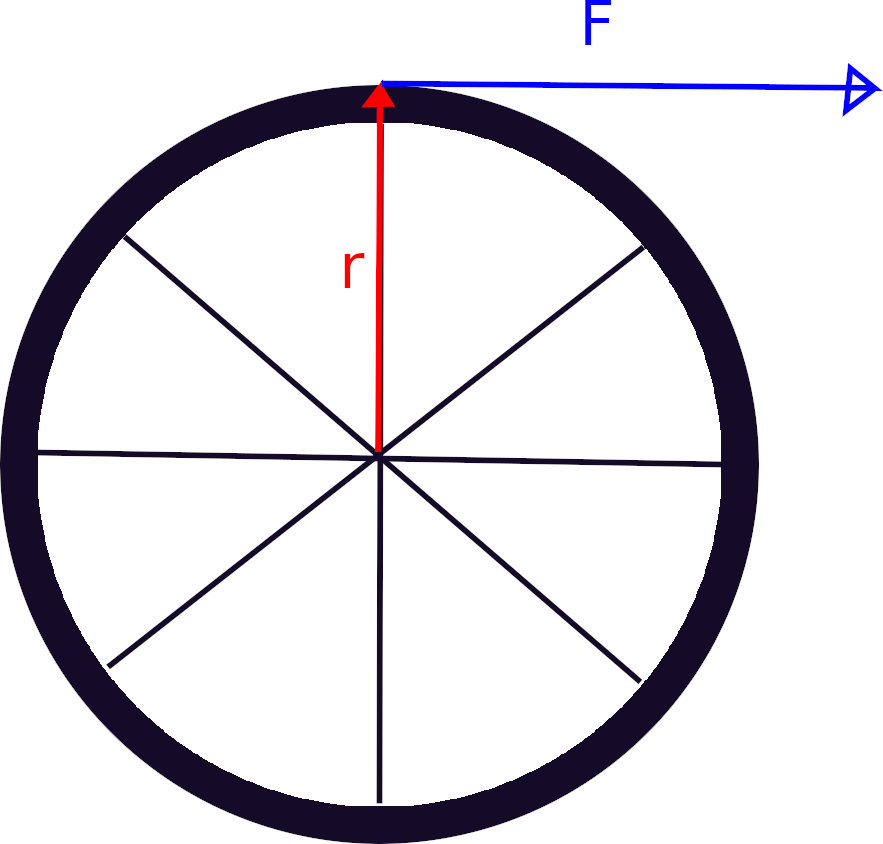
\includegraphics{"./Chapters/Ch09-RotationalMechanics/wheel.png"}
		\vspace{0.1in}
		
		We can use Equation \ref{equation:torquemagnitude} to determine the torque:
		\begin{equation*}
			|\vec{\tau}| = r \cdot F \cdot sin (\theta) = 0.1 \si{m} \cdot 10 \si{N} \cdot \sin( 90 \degree) = \boxed{1 \si{m \times N}}
		\end{equation*}
		
		The direction of the torque is given by the 1st right hand rule.  Your index finger points along the direction of $\vec{r}$.  Your middle finger bends 90 degrees and aligns with $\vec F$.  Your thumb shows the resulting direction of the torque: \textbf{into the page.}
		
	\end{mdframed}
	
	
	
	
	
	
	
	\subsection{Newton's Laws in a Rotational Setting}
	\index{Newton's Laws, Rotational}
	
	\subsubsection{Newton's First Law for Rotation}
	Objects in uniform rotational motion will remain in uniform rotational motion and objects at rotational rest will remain at rotational rest until acted upon by an external, unbalanced torque.  
	
	\subsubsection{Newton's Second Law for Rotation}
			\begin{mdframed}[backgroundcolor=orange!20!white]
		\begin{equation}
			\vec{\tau} = I \cdot \vec{\alpha}
			\label{equation:newtonssecondrotational}
		\end{equation}
	\end{mdframed}
	
	\subsubsection{Newton's Third Law for Rotation}
	For every torque, there is an equal opposite torque.
	
	
	\section{Angular Kinetic Energy}
	\index{Angular Kinetic Energy}
	\textbf{Angular Kinetic Energy}, sometimes called rotational kinetic energy, is energy of rotational motion.  An object that is only rotating - like a fan - has angular kinetic energy only.  An object that is rolling - like the wheel of a car - has both translational kinetic energy (found using $k = \frac{1}{2}mv^2$ ) and angular kinetic energy, found using:
	
				\begin{mdframed}[backgroundcolor=orange!20!white]
		\begin{equation}
			K = \frac{1}{2}I\omega^2
			\label{equation:rotationalkineticenergy}
		\end{equation}
	\end{mdframed}
	
	\newpage
	\section{Angular Momentum} \label{angularmomentum} \index{Angular Momentum}
	\subsection{The Definition of Angular Momentum}
	Angular momentum can be calculated using the formula: 
	 	\begin{mdframed}[backgroundcolor=orange!20!white]
		\begin{equation}
		\vec{L} = I \vec{\omega}
		\label{equation:angularmomentum}
				\end{equation}
	\end{mdframed}
where $\vec{L}$ is angular momentum, $I$ is the object's moment of Inertia and $\vec{\omega}$ is the object's angular velocity.  The SI units for angular momentum are  $\frac{kg m^2} {s} $.


\begin{mdframed}[backgroundcolor=blue!10!white]
	\begin{center}
		
		
		\textbf{Example \thesection.1}	
	\end{center}
	\vspace{0.1in}
	\textbf{Problem:} A bicycle wheel has a mass of 0.3 kg, and can be thought of as a thin ring with a radius of 0.33m. When the wheel is turning at a rate of 2 rotations per second, what its its angular momentum?
	\vspace{0.1in}
	
	\textbf{Solution:} 
	Begin by converting the angular velocity $\omega$ to appropriate units:
	\begin{equation*}
	\vec{\omega} = 2 \frac{rotations}{s} = 4\pi \frac{rad}{s}
	\end{equation*}
	
	Then calculate the moment of inertia.  Using the formula for a thin ring: 
	\begin{equation*}
	I  = mr^2 = 0.3 kg  (0.33m)^2 \approx 0.033 kg m^2
	\end{equation*}
	Finally, use equation \ref{equation:angularmomentum} to find the angular momentum. 
	
	\begin{equation*}
	\vec{L}  =  I \vec{\omega} = 0.011 kg m^2 \cdot 4\pi \frac{rad}{s} \approx \boxed{0.411 \frac{kg m^2}{s}}
	\end{equation*}
	
	
	
\end{mdframed}


	\subsection{Conservation of Angular Momentum}
 Just like linear momentum\footnote{see momentum in \cref{angularmomentum}}, angular momentum is a quantity that is conserved.  Thus, whatever angular momentum a closed system has in its initial state will be equal to the angular momentum the system has in its final state.  
 
 The classic example of the Law of Conservation of Momentum is an ice skater who enters a spin.  By changing the positioning of his or her arms and legs, an ice skater can change their moment of inertia.  When they bring their arms and legs closer to their axis of rotation, their moment of inertia decreases.  Since angular momentum is conserved, their angular velocity must increase as their moment of inertia decreases, and thus the ice skater is able to spin very fast. 
 
	
	

		


	


